\chapter{AirIMU: Learning Uncertainty Propagation for Inertial Odometry} \label{chapter:airimu}
\fancyhead[LO]{\makebox[\textwidth][r]{Chapter 4. AirIMU}}

\section{Introduction}

Inertial Measurement Unit (IMU), capable of sensing high-frequency linear acceleration and angular velocity, is an essential component in almost all kinds of robots \cite{zhao2023subt, burri2016euroc, KITTIDataset}.
As a result, inertial odometry (IO), which aims to estimate the relative movements of robots using IMU measurements, has broad applications in autonomous driving \cite{KITTIDataset}, navigation \cite{qi2002direct}, augmented reality \cite{hincapie2015gyrowand}, and human motion tracking \cite{menolotto2020motion}.
Due to the IMUs' relative independence from the external environment, IO is insensitive to environmental disturbances such as illumination changes and visual obstructions \cite{zhao2023subt}. 
Therefore, IO has great potential in robust state estimation under complex operation conditions, especially compared to exteroceptive sensors like cameras and LiDAR \cite{qin2018vins}.
Nevertheless, the performance of existing IO algorithms, either the model-based \cite{forster2015imu} or the data-driven methods \cite{chen2018ionet}, is still unsatisfactory for real-world applications \cite{zhao2023subt}.


\begin{figure*}[!t]
	\centering
    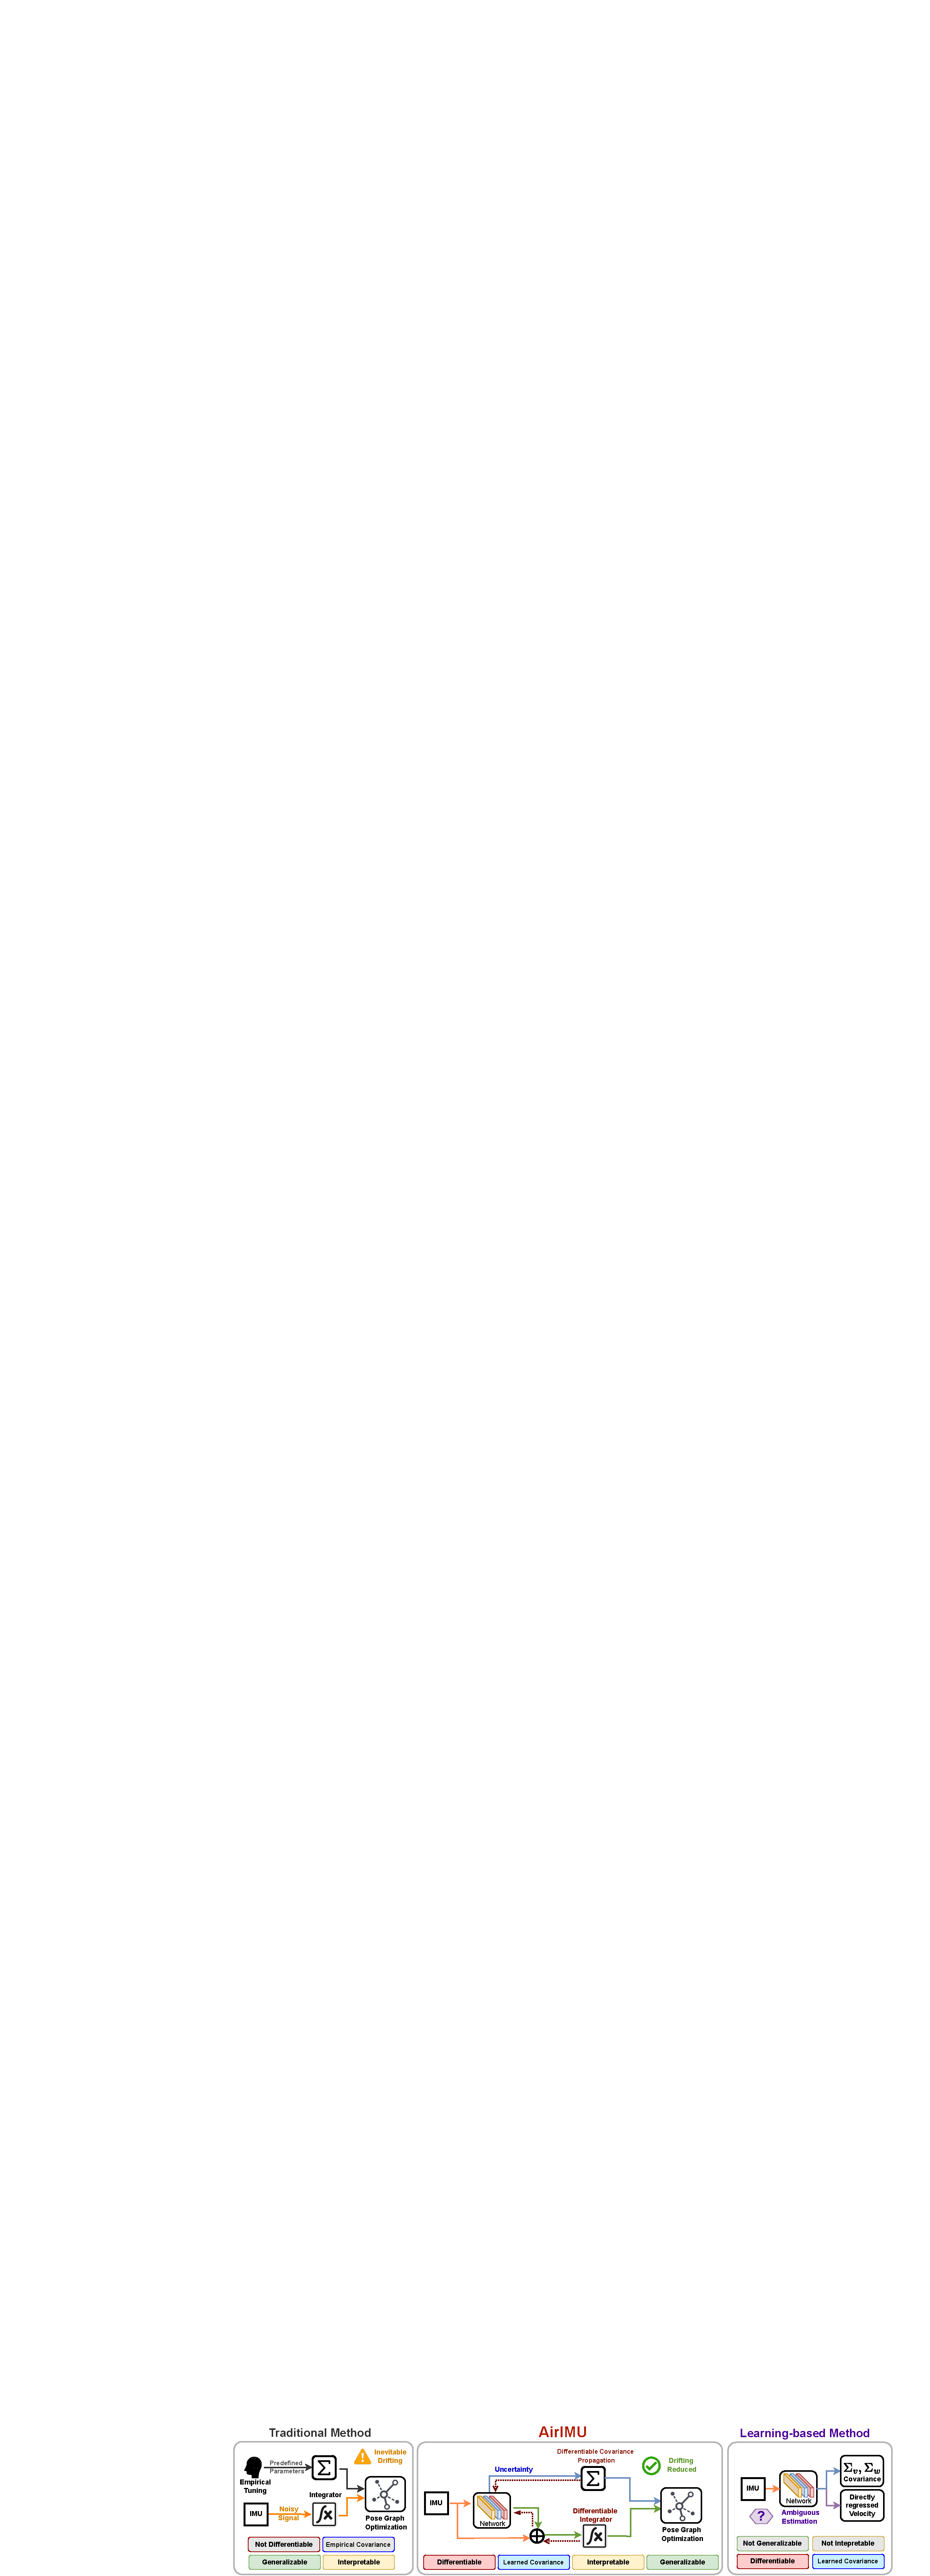
\includegraphics[width=\linewidth]{tex/ch4_airimu/figs/Figure1.pdf}
    \caption{
        % Drift in IMU preintegration is inevitable due to sensor noise. 
        \textbf{Left:} Traditional methods with empirically set uncertainty parameters often fail to capture noise inherent in the sensor accurately.
        \textbf{Middle:} AirIMU corrects the IMU noise and predicts the corresponding uncertainty of the integration. Notably, its covariance propagation is differentiable, promoting efficient training.
        \textbf{Right:} Learning-based methods predict velocity and the corresponding covariance but lack interpretability and generalizability across different data domains.}
	\label{Fig:1}
\end{figure*}



Kinematic model-based IO methods have excellent generalizability but often suffer from complex and multifaceted noise \cite{barshan1995inertial}.
The IMU sensor noises can be classified into two categories: the deterministic errors and the non-deterministic errors \cite{rehder2016extending}.
The deterministic errors are the systematic biases in the measurements that can be consistently predicted or modeled, often arising from factors such as installation imperfections, and calibration errors \cite{li2022calib}.
Conversely, the non-deterministic errors, which are also known as stochastic errors, are related to factors like mechanical shocks, vibration influences, thermal effects, mechanical defects, and calculation ambiguities \cite{jao2023prio, capriglione2020experimental, li2014online}.
%, are classified as non-deterministic errors or sometimes stochastic errors. 
Many methods employ linearized models to handle the deterministic errors by accounting for additive sensor bias, scale factors, and axis misalignment \cite{tedaldi2014robust, furgale2013unified, Krebs2012} and handle non-deterministic errors using zero-mean Gaussian function \cite{qin2018vins, rehder2016extending}.
However, these simplified linear models struggle to fully account for non-deterministic uncertainties from the natural environments, highlighting a critical area for improvement.
Data-driven IO, which use neural networks to predict the motion and implicitly fit the IMU noise, often face challenges with interpretability and generalizability.
To be more specific, these methods often overfit in specific motion patterns such as pedestrian \cite{herath2020ronin} or vehicle \cite{brossard2020ai}, and fail to generalize to scenarios outside of the training distribution.
For example, the model trained on hand-held platforms running on flat ground fails to generalize to robots climbing stairs or drones \cite{buchanan2022deep}.
Moreover, replacing the motion models with the neural networks undermines the model's interpretability.

Recent advances in hybrid methods show the potential to merge the benefits of both the model-based method and the data-driven method. 
For example, some researchers fuse the data-driven motion model with the IMU kinematic motion model using EKF \cite{liu2020tlio, sun2021idol} or batched optimization \cite{buchanan2022learning}.
These solutions improve the robustness of the state estimation but still struggle with generalizability.
On the other hand, efforts have been made in training neural networks to model the error in gyroscope \cite{brossard2020ai}, accelerometer\cite{zhang2021imu}, IMU bias evolution \cite{buchanan2022deep}.
Despite these advancements, none of these algorithms explicitly model the uncertainty of the IMU measurements in the IMU pre-integration.
When deploying the data-driven model with visual-inertial odometry \cite{zhang2021imu, buchanan2022deep}, these algorithms still assume the IMU covariance model as a manually calibrated stochastic variable.
These gaps hinder the deployment of hybrid methods for real-world robots.

To close these gaps, we present a hybrid method AirIMU as illustrated in \fref{Fig:2}. It leverages the data-driven method to model the non-deterministic noise and the kinematic motion model to ensure generalizability in novel environments.
To empower the AirIMU with the ability to learn the uncertainty and noise model, we build a differentiable IMU integrator and a differentiable covariance propagator on manifolds.
Unlike the previous data-driven covariance prediction models \cite{liu2020tlio, sun2021idol} that only predict the covariance of the output translation within a fixed window, we predict the accumulated covariance for a long-time pre-integration.
Moreover, we jointly train the uncertainty module with the noise correction module, which can capture better IMU features and benefit both tasks.

In the experiments, we demonstrate the adaptability to a full spectrum of IMUs encompassing various grades and modalities, as illustrated in \fref{Fig:Devices}.
To validate the effectiveness of our learned covariance in sensor fusion, we design a pose graph optimization (PGO) system that fuses the AirIMU outputs with the GPS signals. 
To the best of our knowledge, we are the first to train a deep neural network that models IMU sensor uncertainty through differentiable covariance propagation.
In summary, the main contributions of this paper are:
\begin{itemize}

\item This paper proposes AirIMU, a hybrid method that leverages the data-driven method to model the non-deterministic error, and the kinematic motion model to ensure generalizability in novel environments. 

\item We propose to jointly train the IMU noise and uncertainty through the differentiable integrator and covariance propagator.
This training strategy improves 17.8\% of the IMU preintegration results in Subt-MRS benchmark \cite{zhao2023subt}.

\item Our method demonstrates adaptability across multiple grades of IMUs, from low-cost automotive-grade IMUs to high-end navigation-grade IMUs.
We further evaluate AirIMU on the large-scale visual terrain navigation dataset ATLO \cite{cisneros2022alto} cruising over 262 \si{\km}.
Additionally, we illustrate the effectiveness of the learned uncertainty in a GPS-IMU PGO experiment, achieving a 31.6\% improvement in optimization.

\item We develop a tool package for the differentiable IMU integrator and covariance propagator that supports batched operations and the cumulative product, which speeds up the training process.
This package is grounded on \textit{PyPose} \cite{wang2023pypose} library and the tutorial is now open-source at:  \href{https://pypose.org/tutorials/imu/imu_integrator_tutorial}{https://pypose.org/tutorials/imu}

\end{itemize}

\section{Related Works}

\subsection{Traditional Inertial Odometry}
\label{sec: imu-denoise}
Traditional model-based IO algorithms utilize the IMU kinematic motion model \cite{forster2015imu} to estimate the relative motion and are often integrated with other auxiliary sensors like GPS, Camera \cite{qin2018vins}, and LiDAR \cite{hemann2016long} with filter-based method or batched optimization.
To deploy IO on mobile robots, especially those equipped with low-cost IMUs, modeling IMU deterministic errors is indispensable \cite{barshan1995inertial}, which generally include the additive sensor bias, scale factors, and axis misalignment \cite{rehder2017camera}. 

To address the non-deterministic error, factors like nonlinearity, g-sensitivity \cite{Krebs2012}, size effect \cite{hung1979size}, vibration \cite{capriglione2020experimental}, thermal effect \cite{niu2013fast}, and Coriolis force \cite{brossard2021associating} are rigorously addressed.
These methods, however, rely on expensive motion simulators such as shakers and rate tables \cite{qureshi2017algorithm}, which is not available in practice.
To calibrate the low-cost IMUs, the IO algorithms utilize the IMU measurements under static conditions \cite{tedaldi2014robust, barshan1995inertial}, or auxiliary sensors like the camera \cite{rehder2016extending, yang2023online} and LiDAR \cite{lv2020targetless} for calibration.
Kalibr \cite{rehder2016extending} is one of the most widely used calibration algorithms, calibrating the IMU intrinsic and extrinsic parameters between the camera and the IMU.
However, all these calibration methods focus on modeling the linear behavior of the IMU sensor under static conditions or controlled environments, which often struggle to fully capture the noise inherent in the natural environment and sensor defects.
This reveals a significant gap in the current IMU calibration and the practices of IO.

\subsection{Learning Inertial Odometry}
\label{Sec: LIO}
A growing trend in leveraging a data-driven model for IO has been witnessed, such as IMU odometry network \cite{yan2018ridi, chen2018ionet}, EKF-fused IMU odometry \cite{liu2020tlio, sun2021idol, cao2022rio} and learning-based IMU calibration \cite{brossard2020denoising}.
In RIDI \cite{yan2018ridi}, a supervised Support Vector Machine (SVM) classifier is introduced to determine IMU placement modes (e.g., handheld, bag) using accelerometer and gyroscope measurements.
Mode-specific Support Vector Regressions (SVRs) are then employed to estimate pedestrian velocities based on motion types, enabling corrective adjustments to sensor readings.
IONet \cite{chen2018ionet} introduced deep learning to regress the translation within a fixed temporal window. 
Building on this concept, RoNIN \cite{herath2020ronin} improves the accuracy of the data-driven IO with multiple neural network architectures, including Temporal Convolutional Networks (TCN) and Long Short-Term Memory (LSTM).
RIO \cite{cao2022rio} explores rotation-equivalence as a self-supervisory mechanism for training IO models. 
These studies utilize data-driven motion estimation models to replace the IMU integration process, thereby reducing the drift associated with IMU double integration. 
Inspired by these IMU odometry network studies, TLIO \cite{liu2020tlio} integrates the data-driven motion estimation model with the IMU integrator through a stochastic-cloning Extended Kalman Filter (EKF). 
This integrated approach optimizes position, orientation, and sensor biases, solely with IMU data.
IDOL \cite{sun2021idol} further extends this framework with a data-driven orientation estimator, generating more accurate results with better consistency.
% These strategies train neural networks to model the IMU kinematics function, which, as a result, lacks an accuracy guarantee in relative pose estimation compared to IMU integration.
Although these methods are promising in pedestrian datasets like RoNIN \cite{herath2020ronin}, the motion estimation heavily relies on prior knowledge about human movements, such as the consistent walking pattern of pedestrians and constant velocity assumption, which fail to generalize to other platforms like drones and vehicles.
Moreover, these studies often assume the IMU measurement is transformed to the world coordinates or aligning the y-axis with gravity, which is impractical in real scenarios. 

Inspired by the advancements of the data-driven methods in modeling unknown parameters, prior researchers employ neural networks to implicitly calibrate the IMUs \cite{nobre2019learning, brossard2020denoising, zhang2021imu}. 
Brossard et al. \cite{brossard2020denoising} train a Convolutional Neural Network (CNN) to denoise the low-frequency error in gyroscopes.
Zhang et al. \cite{zhang2021imu} employed a Long Short-Term Memory (LSTM) network to preprocess the raw IMU, and subsequently channeled the preprocessed IMU measurements into a filter-based visual-inertial odometry system.
Deep IMU Bias \cite{buchanan2022deep}, utilizes neural networks to model the sensor bias, and incorporates the learned bias as an additional constraint in the bundle adjustment.
These studies showcase the potential of data-driven methods in modeling IMU errors, especially when the sensor's physical conditions are difficult to capture.
However, none of the referenced algorithms have explicitly tackled the challenge of modeling the uncertainty for IMU integration.
When deploying these data-driven models, the predefined covariance parameters can no longer fit the learned IMU sensor model, undermining the IO's accuracy and robustness. 

\begin{figure}[!t]
	\centering
    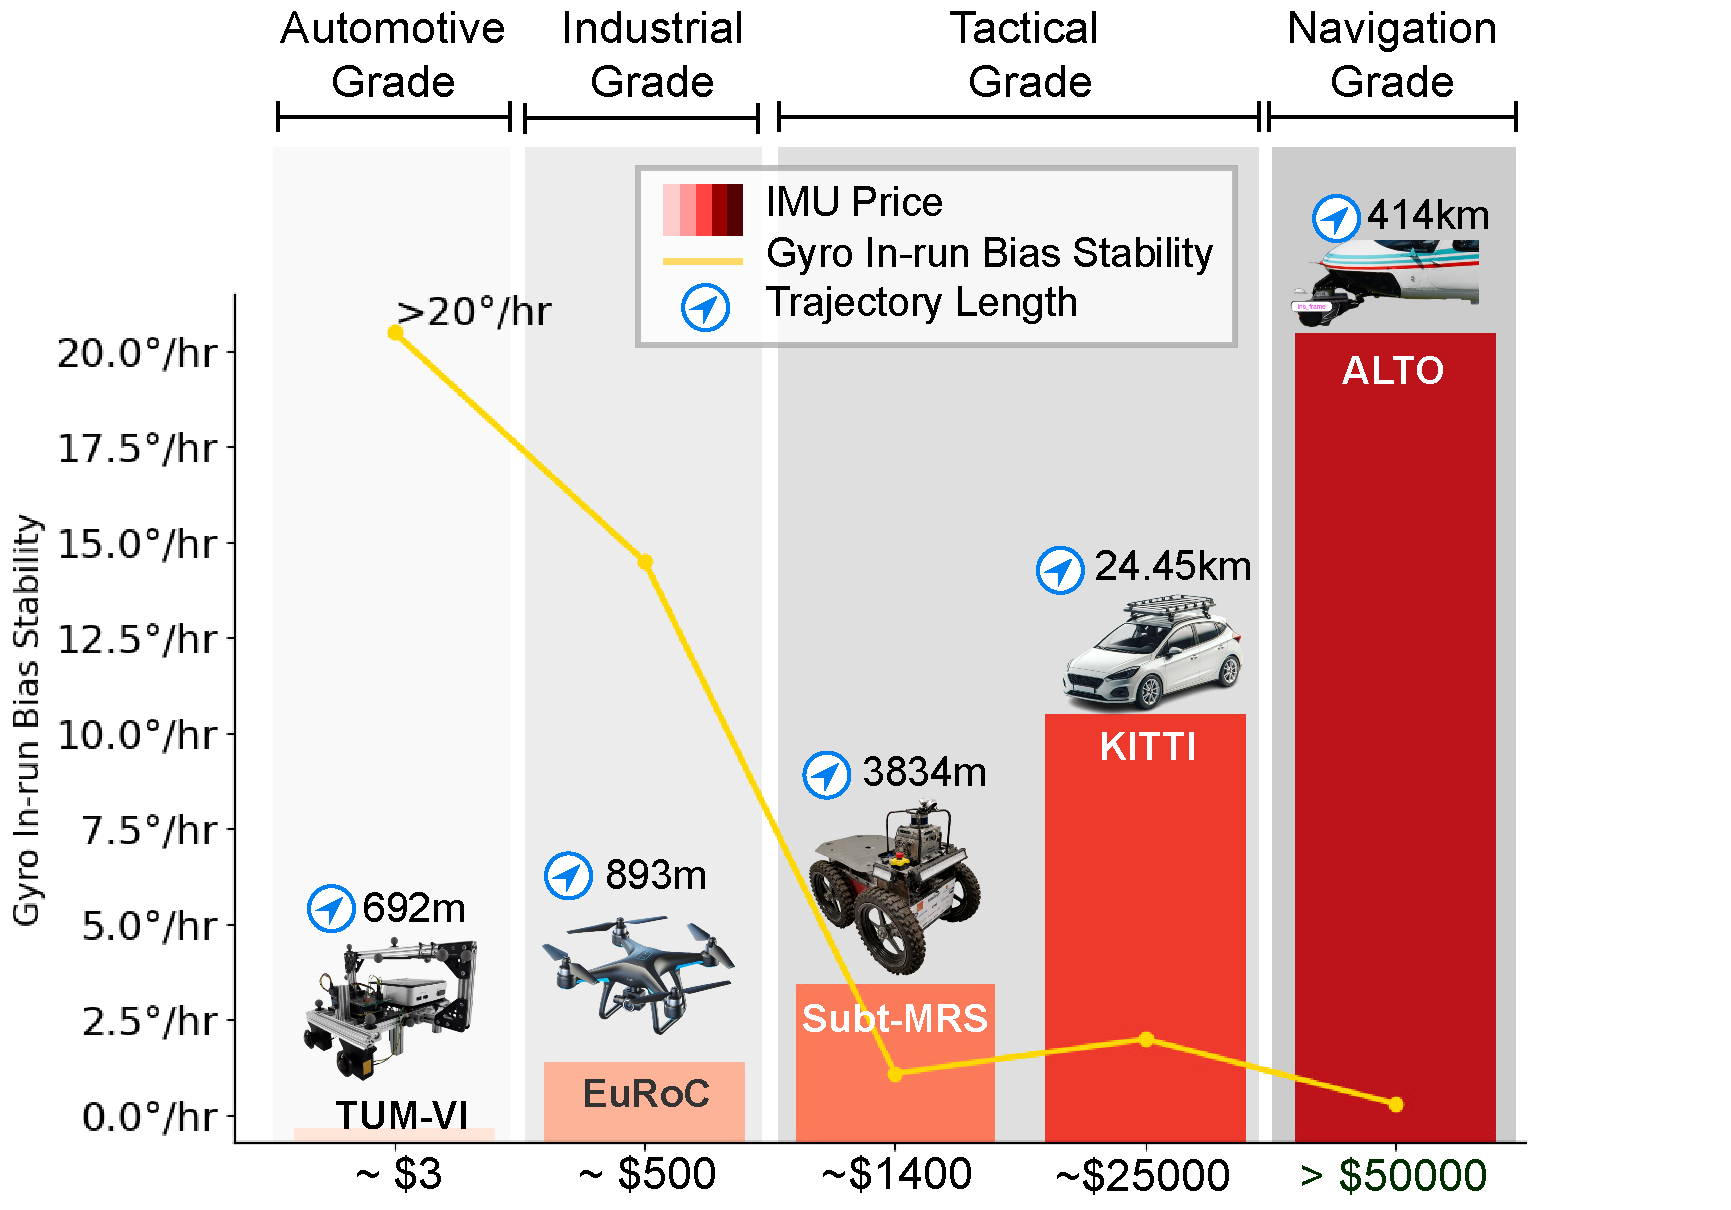
\includegraphics[width=0.95\linewidth]{tex/ch4_airimu/figs/imudevice.pdf}
    \caption{
        We evaluate our algorithm on IMUs with different prices and drift rates. Sensor quality is evaluated based on the gyroscope's in-run bias stability metric. Our evaluation spans the full spectrum of IMUs, including automotive-grade, industrial-grade, tactical-grade, and navigation-grade IMUs.}
	\label{Fig:Devices}
\end{figure}


\subsection{IMU uncertainty model}
% One key challenge in IO is the covariance model of the IMU sensor.
The uncertainty model in IO, which quantifies the reliability of inertial measurements, is the key to optimizing both filter performance and the batched optimization results. 
Traditional IO follows the kinematics model formulated in the IMU integration to propagate the covariance matrix from the predefined IMU uncertainty parameters \cite{forster2015imu}.
A commonly used solution to calibrate the uncertainty parameters is the Allen deviation \cite{el2007analysis}, which quantifies the sensor bias and bias instability by analyzing the variance of the sensor errors in a static position.
However, these parameters often require empirical tuning and manual re-calibration during testing due to unknown environmental disturbances and mechanical imperfections.

Recent researches in data-driven methods demonstrate the potential to model the uncertainty model with neural network \cite{russell2021multivariate}.
% Another strategy is to predict the uncertainty with the neural network in the state estimation \cite{russell2021multivariate}.
The AI-IMU \cite{brossard2020ai} proposes a dead-reckoning algorithm for vehicles, which assumes that the lateral and vertical velocities are approximately null.
To model the confidence degree of these null assumptions, the authors train a CNN network from IMU to predict two constant uncertainty parameters corresponding to lateral and vertical velocity.
DualProNet \cite{solodar2023vio} is another attempt to use a deep neural network to predict the uncertainty parameters in IMUs.
This work, however, requires high-frequency ground truth covariance labels for all IMU measurements, which are generally non-available during practice.
In TLIO \cite{liu2020tlio}, the authors jointly train a covariance model of the predicted velocity with a fixed temporal window, which is later fused in an EKF. 

In response to these challenges, our method leverages the differentiable covariance propagation to learn the high data-rate uncertainty. 
This approach alleviates the need for high-frequency ground truth labels and bridges the gap between uncertainty modeling and practical limitations.

\section{AirIMU Model}

% we introduce our AirIMU model in \fref{Fig:2}, consisting of the data-driven and kinematic motion modules.

% To maintain the generalizability, we decouple the kinematic model and the data-driven model for state estimation.
% the AirIMU employs the data-driven model to predict the error and uncertainty in sensor frame rate and uses the kinematic-based integrator and covariance propagator to estimate the state $x$ and covariance $\Sigma$. 
% To decouple the non-deterministic error model from the well-defined kinematic motion model,
To balance the accuracy and generalizability, the AirIMU model decouples the non-deterministic error model from the precisely defined kinematic motion model, as depicted in \fref{Fig:2}. 
Specifically, it utilizes a data-driven model to capture the error and uncertainty inherent in the IMU, while employing the kinematic-based method to integrate the state and covariance.
By supervising the integrated state and covariance, the AirIMU jointly trains the sensor error and uncertainty models throughout the differentiable integrator.
To accelerate the training speed with long sequences, we propose a tree-like structure for cumulative operation and redesign the covariance propagation to facilitate batched operation and parallel computing.
The refined state and covariance outputs are subsequently incorporated into the PGO module, where they are fused with auxiliary sensors such as GPS.
% By supervising the state $x$ and covariance $\Sigma$, the AirIMU jointly trains the sensor error and uncertainty models throughout the differentiable integrator.
% The state $x_k$ includes orientation $R$, velocity $v$, and position $p$ within the reference frame $\{W\}$ in the $k$-th frame.



Overall, we show the data-driven model in \sref{Model: Network}, the kinematic model in \sref{Model: Integrator}, loss functions in \sref{Model: Loss}.
Moreover, we detail our efforts of accelerating the integration and covariance propagation in \sref{Model: Accelerate}. Lastly, we present the PGO module that fuses the AirIMU with auxiliary sensors like GPS in \sref{Model: System}.

\subsection{Data-driven module}
\label{Model: Network}
\begin{figure}[!t]
	\centering
    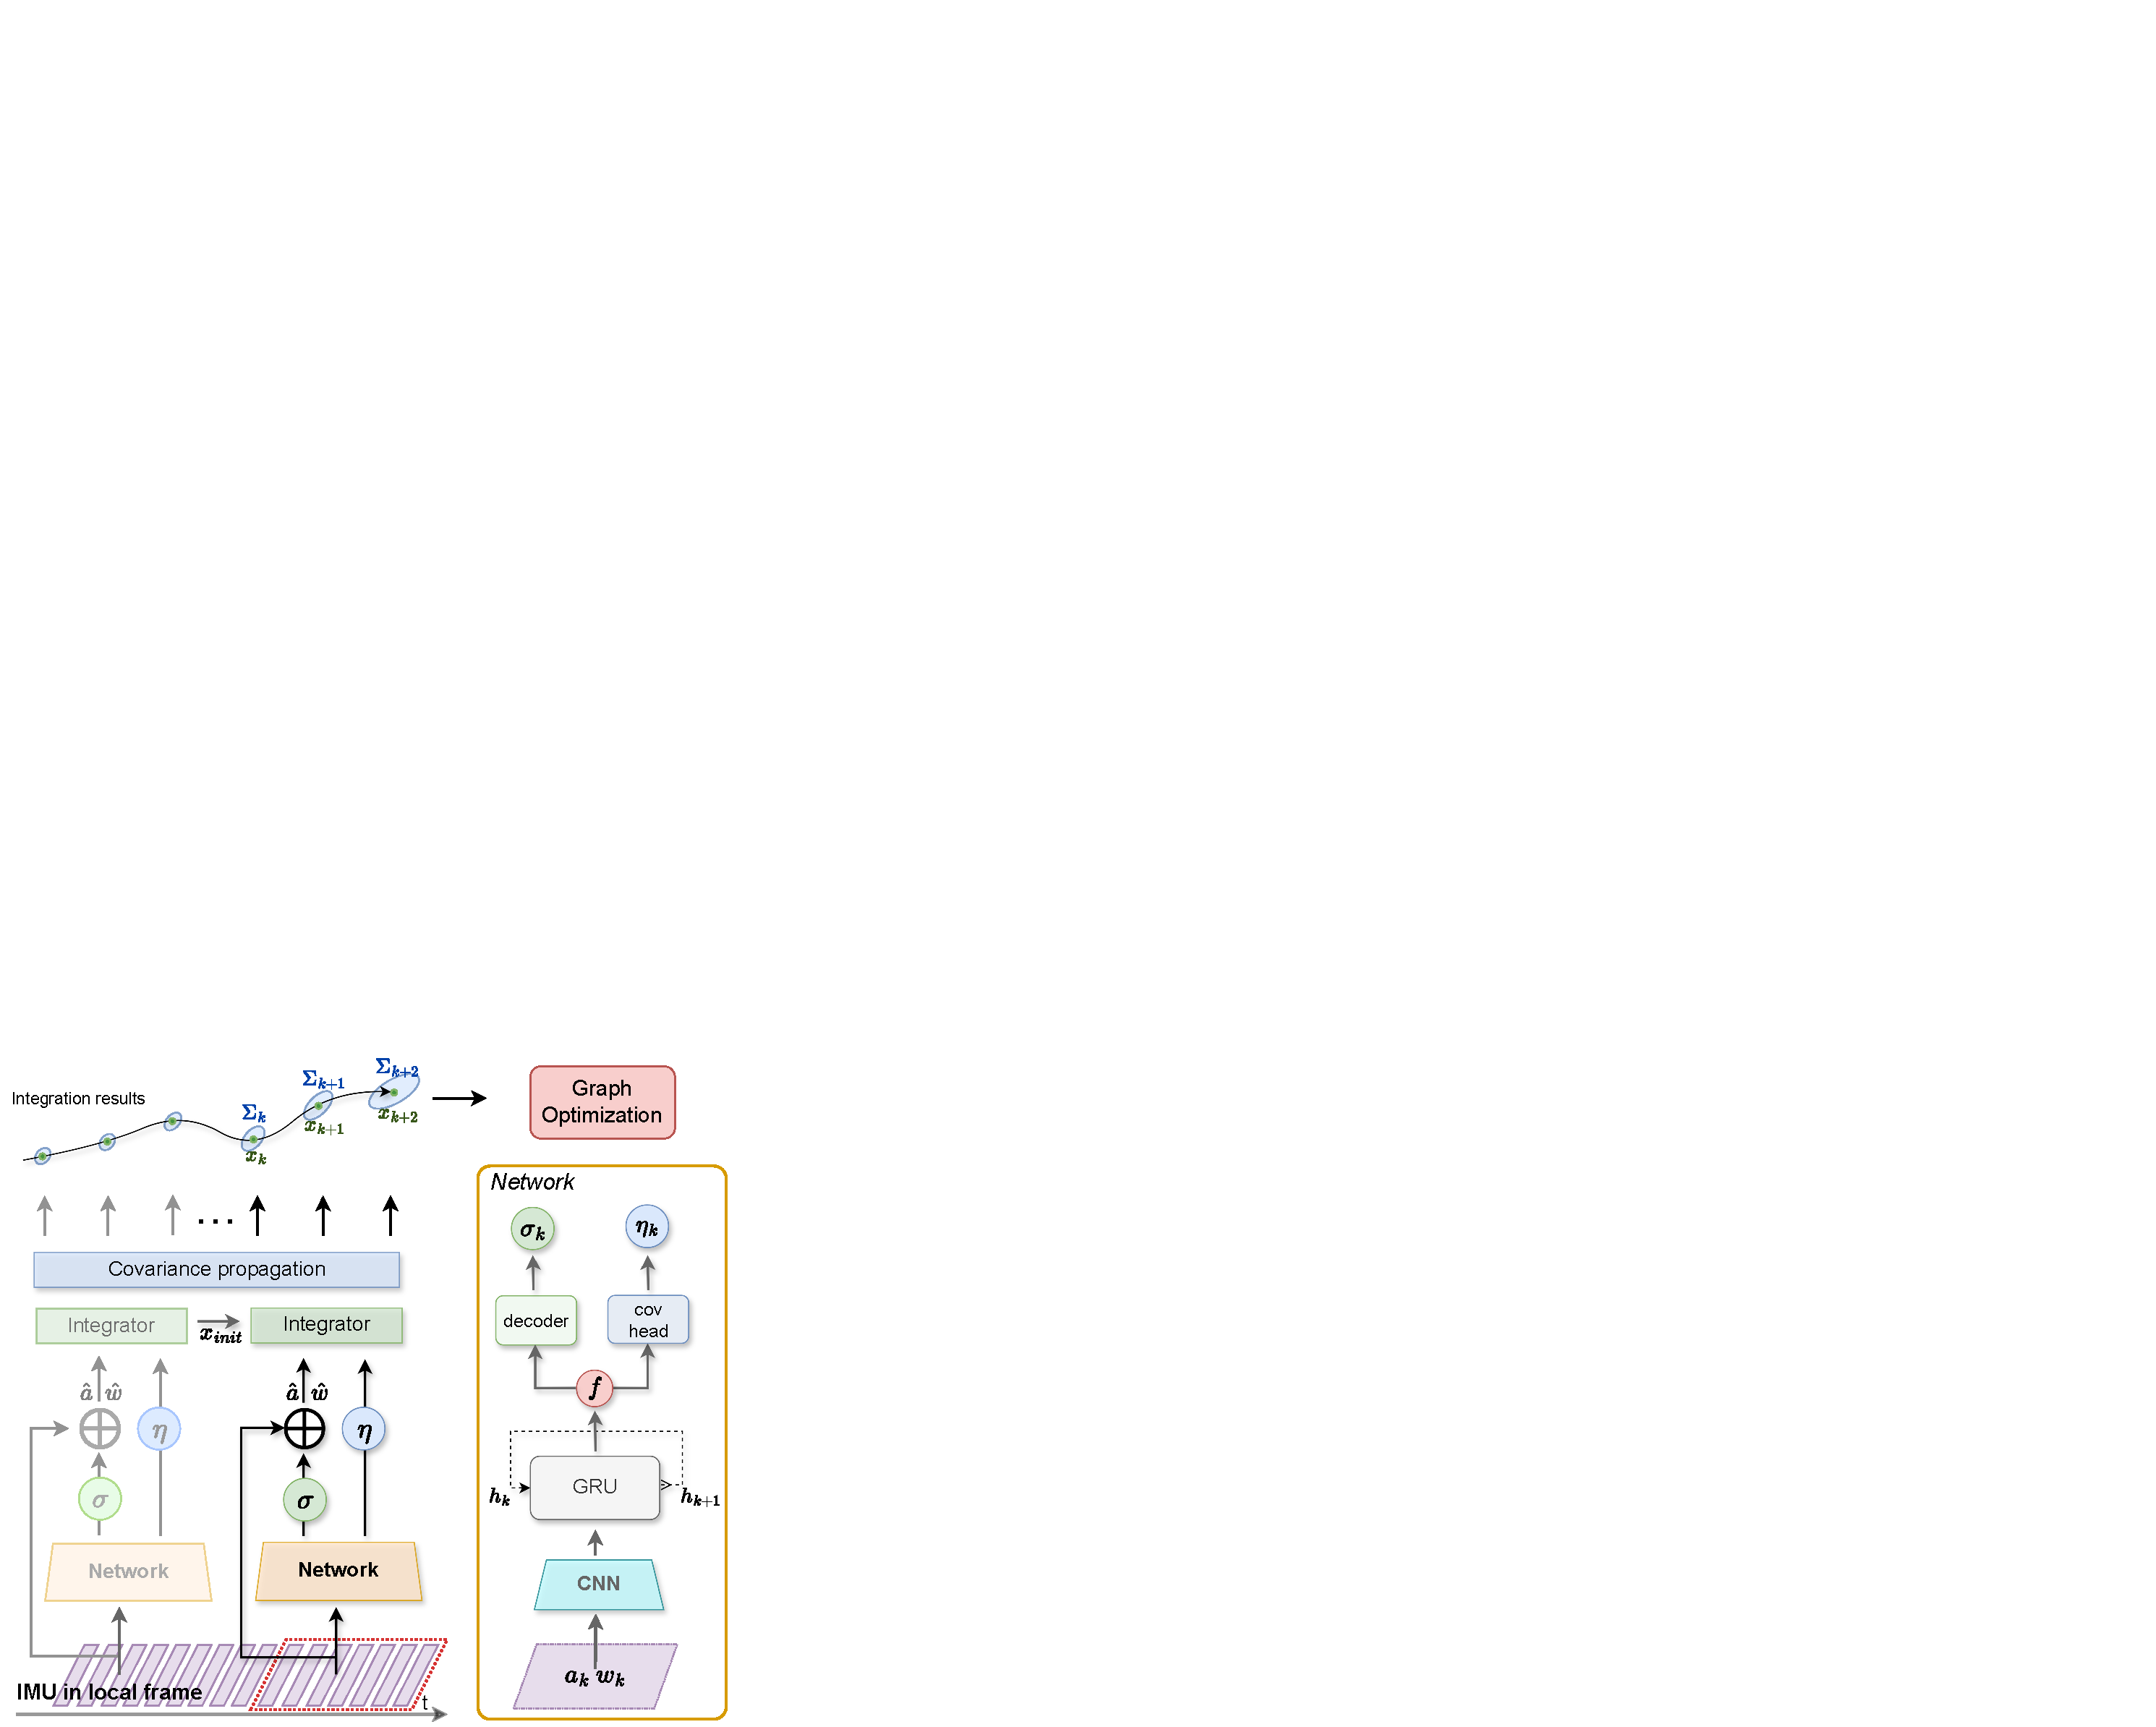
\includegraphics[width=\linewidth]{tex/ch4_airimu/figs/Figure2.pdf}
    \caption{
    \textbf{Right:} We employ a CNN-GRU encoder to capture IMU features ($f$) from raw IMU accelerometer ($a_k$) and gyroscope ($w_k$) measurements.
    Subsequently, these features are decoded to obtain IMU corrections ($\sigma_{acc}$, $\sigma_{gyro}$).
    \textbf{Left:} We add the raw measurements with learned corrections, generating corrected IMU measurements ($\hat a_k$ and $\hat w_k$). The learned uncertainties ($\eta$) are propagated to estimate the corresponding covariance matrix ($\Sigma$).
}
	\label{Fig:2}
\end{figure}
% Many existing data-driven inertial algorithms presume that ground truth orientations are available to transform the raw input from the IMU sensor frame to world frame $\{W\}$ or a Heading-Agnostic Coordinate Frame (HACF) defined in \cite{herath2020ronin}.
% However, the ground truth orientation may not be available in real-world applications.


% After applying the sensor model, we denote the corrected acceleration as ${}^B{\tilde a}$ and the angular velocity as ${}^B{\tilde w}$.
As shown in the right part of \fref{Fig:2}, the AirIMU model utilizes an encoder-decoder network structure to process raw IMU data, which includes three-axis acceleration $a$ and three-axis angular velocity $w$, both measured in the body frame ${B}$. The network outputs corrections for acceleration and angular velocity, denoted as ${}^B\sigma^{acc}$ and ${}^B\sigma^{gyro}$, respectively. Additionally, it calculates the corresponding uncertainty measures for the gyroscope $\eta^{gyro}$ and accelerometer $\eta^{acc}$.

To leverage and understand the hidden relationship between the IMU noise and uncertainty, we train a shared encoder network to capture the common representations of the raw IMU measurements for both tasks.
% from the IMU body frame $\{B\}$.
% The network comprises an encoder and decoder structure.
In the encoder model, we first utilize a 1D CNN network to learn the lower-level features like the pattern of the accelerometer and gyroscope.
To capture the temporal dependency from the previous IMU data, we combine the CNN network with gated recurrent unit (GRU) layers to generate the IMU feature.
% responsible for encoding the raw input acceleration ${}^B a$ and angular velocity ${}^B w$.

With the shared features, we build a correction decoder to estimate the error ${}^B{\sigma^{gyro}}, {}^B{\sigma^{acc}}$ in the following:
\begin{equation}
    \left[{}^B{\sigma^{gyro}}, {}^B{\sigma^{acc}}\right] = f_\pi\left({}^Bw, {}^Ba\right),
\end{equation}

where $\pi$ represents the learnable parameters of the decoder. 
For the covariance, we train another decoder with a similar structure to predict the uncertainty of each corresponding frame. 
This uncertainty is predicted by a covariance model denoted as:
\begin{equation}
    \left[\eta^{gyro}, \eta^{acc}\right] = \Sigma_\theta\left({}^Bw, {}^Ba\right), 
\end{equation}
where $\theta$ represents the learnable parameters of the covariance decoder model.
% , which predicts the uncertainty of the IMU pre-integration in each frame $k$. 

Overall, the corrected acceleration and angular velocity ${}^B{\tilde a}$ and ${}^B{\tilde w}$, are formulated as the summation of the original input ${}^Ba. {}^Bw$, the network corrections ${}^B{\sigma_{acc}}, {}^B{\sigma_{gyro}}$, and noise of the measurements:
\begin{equation}
    {}^B{\tilde a} = {}^Ba + {}^B{\sigma_{acc}} + \eta^{acc}_k,\  {}^B{\tilde w} = {}^Bw + {}^B{\sigma_{gyro}}  + \eta^{gyro}_k.
\end{equation}
Combined with these outputs with the learned uncertainty $\eta^{gyro}_k, \eta^{acc}_k$, we utilize the IMU kinematic model to estimate the states ${}^Wx_j$, and more importantly, to propagate the corresponding covariance $\Sigma_{i,j}$.

\subsection{Differentiable Integration and Covariance Module}
\label{Model: Integrator}
Labeling the ground truth of the high-frequency data requires expensive motion simulators, which is infeasible due to the cost.
Therefore, AirIMU builds a differentiable integrator and covariance propagator to supervise the data-driven module throughout the integration and covariance propagation. 

The IMU pre-integration follows Newton's kinematic laws, which are well-defined in \cite{forster2015imu}. 
The integrated state $x_k$ includes orientation $R$, velocity $v$, and position $p$ within the reference frame $\{W\}$ in the $k$-th frame.
The integration from $i$-th frame to $j$-th frame is formulated as:
\begin{equation}
    \begin{split}
    \label{formula: 2.integrate}
        {\Delta}R_{ij} &= \int_{t \in [t_i, t_j]} {}^B \tilde w_k \ dt \\
        {\Delta}v_{ij} &= \int_{t \in [t_i, t_j]} R_{k} {}^B \tilde a_k \ dt \\
        {\Delta}p_{ij} &= \int\int_{t \in [t_i, t_j]} R_{k} {}^B \tilde a_k\ dt^2\ ,
    \end{split}
\end{equation}
where the ${\Delta}R_{ij}$, ${\Delta}v_{ij}$ and ${\Delta}p_{ij}$ denotes the increments of rotation, velocity and position from frame $i$ to frame $j$ respectively.
Given these increments, the $j$-th state of the robot ${}^Wx_j$ in the world frame $\{W\}$ can be predicted through:
\begin{equation}
    \begin{split}
    \label{formula: 3.predict}
        \tensor[^W]{R}{_j} &= {\Delta}R_{ij} \otimes {}^WR_i \\
        {}^Wv_j &= {}^WR_i * {\Delta}v_{ij}   + {}^Wv_i\\
        {}^Wp_j &= {}^WR_i * {\Delta}p_{ij}   + {}^Wp_i + {}^Wv_i \Delta t_{ij},
    \end{split}
\end{equation}
where the ${}^WR_i$, ${}^Wv_i$, and ${}^Wp_i$ are the state of $i$-th frame.

The propagation of the IMU covariance also follows the IMUs' kinematic model.
Following the conventions established by Forster et al. \cite{forster2015imu}, the covariance of the predicted state is characterized as:
$[\delta \phi_{k}^T, \delta v_{k}^T, \delta p_{k}^T]^T \sim \mathbb{N}(0_{9 \times 1}, \Sigma_{k})$, where the $\delta \phi_{k}$,  $\delta v_{k}$ and $ \delta p_{k}$ represents the zero-mean Gaussian noise for rotation, velocity and position.
We apply a similar covariance propagation strategy as \cite{forster2015imu} to model the covariance matrix $\Sigma_{i,i}$ of the IMU integration from frame i to frame i+1 through iterative propagation. Starting from the initial covariance matrix $\Sigma_{i,i} = 0_{9 \times 9}$, we predict the covariance matrix as:
    \begin{equation}
    \label{formula: 4.cov}
        \Sigma_{i,i+1} 
          = A \Sigma_{i,i} A^T + B_g \mathrm{diag}(\eta^{gyro}_i) B_g^T + B_a \mathrm{diag}(\eta^{acc}_i) B_a^T,
    \end{equation}
where state transition matrix A is defined as:
             \begin{equation}A =
            \begin{bmatrix}
                  {\Delta}R_{kk+1}^T & 0_{3 \times 3}  & 0_{3 \times 3} \\
                  -{\Delta}R_{ik} ({}^Ba_k^{\wedge}) {\Delta}t & I_{3 \times 3} & 0_{3 \times 3} \\
                  -1/2{\Delta}R_{ik} ({}^Ba_k^{\wedge}) {\Delta}t^2 & I_{3 \times 3} {\Delta}t & I_{3 \times 3}
                  \end{bmatrix}.
                \end{equation}
The $B$ matrix addresses the frame-by-frame uncertainty of the acceleration and the angular velocity. 
\begin{equation}
            B_g = \begin{bmatrix}
                    J_r^k \Delta t  \\
                    0_{3 \times 3}  \\
                    0_{3 \times 3} 
                \end{bmatrix}, \ \ \ 
                B_a = \begin{bmatrix}
                    0_{3 \times 3} \\
                    {\Delta}R_{ik} {\Delta}t  \\
                    1/2 {\Delta}R_{ik} {\Delta}t^2
                \end{bmatrix}.
\end{equation}
The covariance matrix is $9 \times 9$ matrix, and we denote it as:

\begin{equation}
\Sigma_{i,j+1} = 
\begin{bmatrix}
\Sigma^r_{i,j+1} & 0_{3 \times 3} & 0_{3 \times 3}\\
0_{3 \times 3} & \Sigma^v_{i,j+1} & 0_{3 \times 3} \\
0_{3 \times 3} & 0_{3 \times 3} & \Sigma^p_{i,j+1} \\
\end{bmatrix},
\end{equation}
where $\Sigma^r_{i,j+1}, \Sigma^v_{i,j+1} \text{and} \Sigma^p_{i,j+1}$ are $3\times 3$ matrix representing the covariance of rotation, velocity, and position respectively.

\subsection{Loss Function and Training strategy}
\label{Model: Loss}

To supervise the learnable model in AirIMU, we design the state loss \eqref{Eq: state loss} for noise correction and covariance loss \eqref{Eq: cov loss} for uncertainty estimation.
Given the differentiable integrator defined in \eqref{formula: 2.integrate} and \eqref{formula: 3.predict}, we train the denoising module $f_\pi(w, a)$ by supervising the state loss with the position, orientation, and translation in the world frame $\{W\}$.
\begin{equation}
\label{Eq: state loss}
    \begin{split}
        L_r &= \| \log({}^W R_i \otimes {}^W \hat R_i) \|_h, \\
        L_v &= \| {}^W v_i -  {}^W \hat v_i \|_h, \\
        L_p &= \| {}^W p_i - \hat {}^W p_i \|_h. \\
    \end{split}
\end{equation}
The $\| \cdot \|_h$ denotes the Huber function, chosen for its robustness in penalizing the large error terms, particularly in lengthy integration sequences.
We transform the orientation error to $\log$ space in the loss function \eqref{Eq: state loss} to supervise the rotation in the manifold, which reduces the single value during training.

To supervise the covariance, we use a similar loss function derived in Russell et al.  \cite{russell2021multivariate}. 
For the covariance of rotation $\Sigma^r_{i,j}$, velocity $\Sigma^v_{i,j}$ and position $\Sigma^p_{i,j}$, we design the covariance losses as:
\begin{equation}
\label{Eq: cov loss}
    \begin{split}
        L^{cov}_r &= \frac{1}{2}\left(\left\|\log({}^WR_j \otimes  {}^W \hat R_j)\right\|^2_{\Sigma^r_{i,j}}  + \ln (\det\Sigma^r_{i,j})\right), \\
        L^{cov}_v &= \frac{1}{2}\left(\left\|{}^Wv_j - {}^W \hat v_j\right\|^2_{\Sigma^v_{i,j}} + \ln (\det \Sigma^v_{i,j})\right), \\
        L^{cov}_p &= \frac{1}{2} \left(\left\|{}^W p_j - {}^W \hat p_j\right\|^2_{\Sigma^p_{i,j}}  + \ln (\det \Sigma^p_{i,j})\right), \\
    \end{split}
\end{equation}
where $y$ is the ground-truth label and $f(w, a)$ output the integrated state. 
The $\Sigma_\theta(x)$ denotes the covariance model that predicts the covariance matrix given the learned uncertainty $\eta$. 
To simplify and stabilize the training process, our training focuses on the diagonal components of the covariance matrix.
The final loss function can be denoted as:
\begin{equation}
L = L_r + L_v + L_p + \varepsilon (L^{cov}_r + L^{cov}_v +L^{cov}_p),
\end{equation}
where we set the weight of the covariance loss as $\varepsilon = 1\times 10^{-3}$.
We chose this parameter to mitigate the impact of relatively small covariance values, which otherwise lead to large covariance losses.

In contrast to previous methods that utilized data augmentation techniques such as random bias and rotation equivalence, we avoid applying data augmentation to sensor model training.
Our approach preserves the original noise in the raw data, which is critical for the AirIMU model to learn the noise pattern in the real sensor.
For most datasets, we set the length of the training segment as 1000 frames (5 seconds). 
This duration allows us to capture both the drift and the long-term features essential for IMU integration.

For the optimizer, we employ the Adam with a learning rate of $1 \times 10^{-3}$ with a weight decay $1 \times 10^{-4}$.
The weighting of each loss term and learning rate may be adjusted to accommodate the specific characteristics of different types of IMU, particularly with different bias instability of gyroscopes and accelerometers.

\begin{figure}[!t]
	\centering
    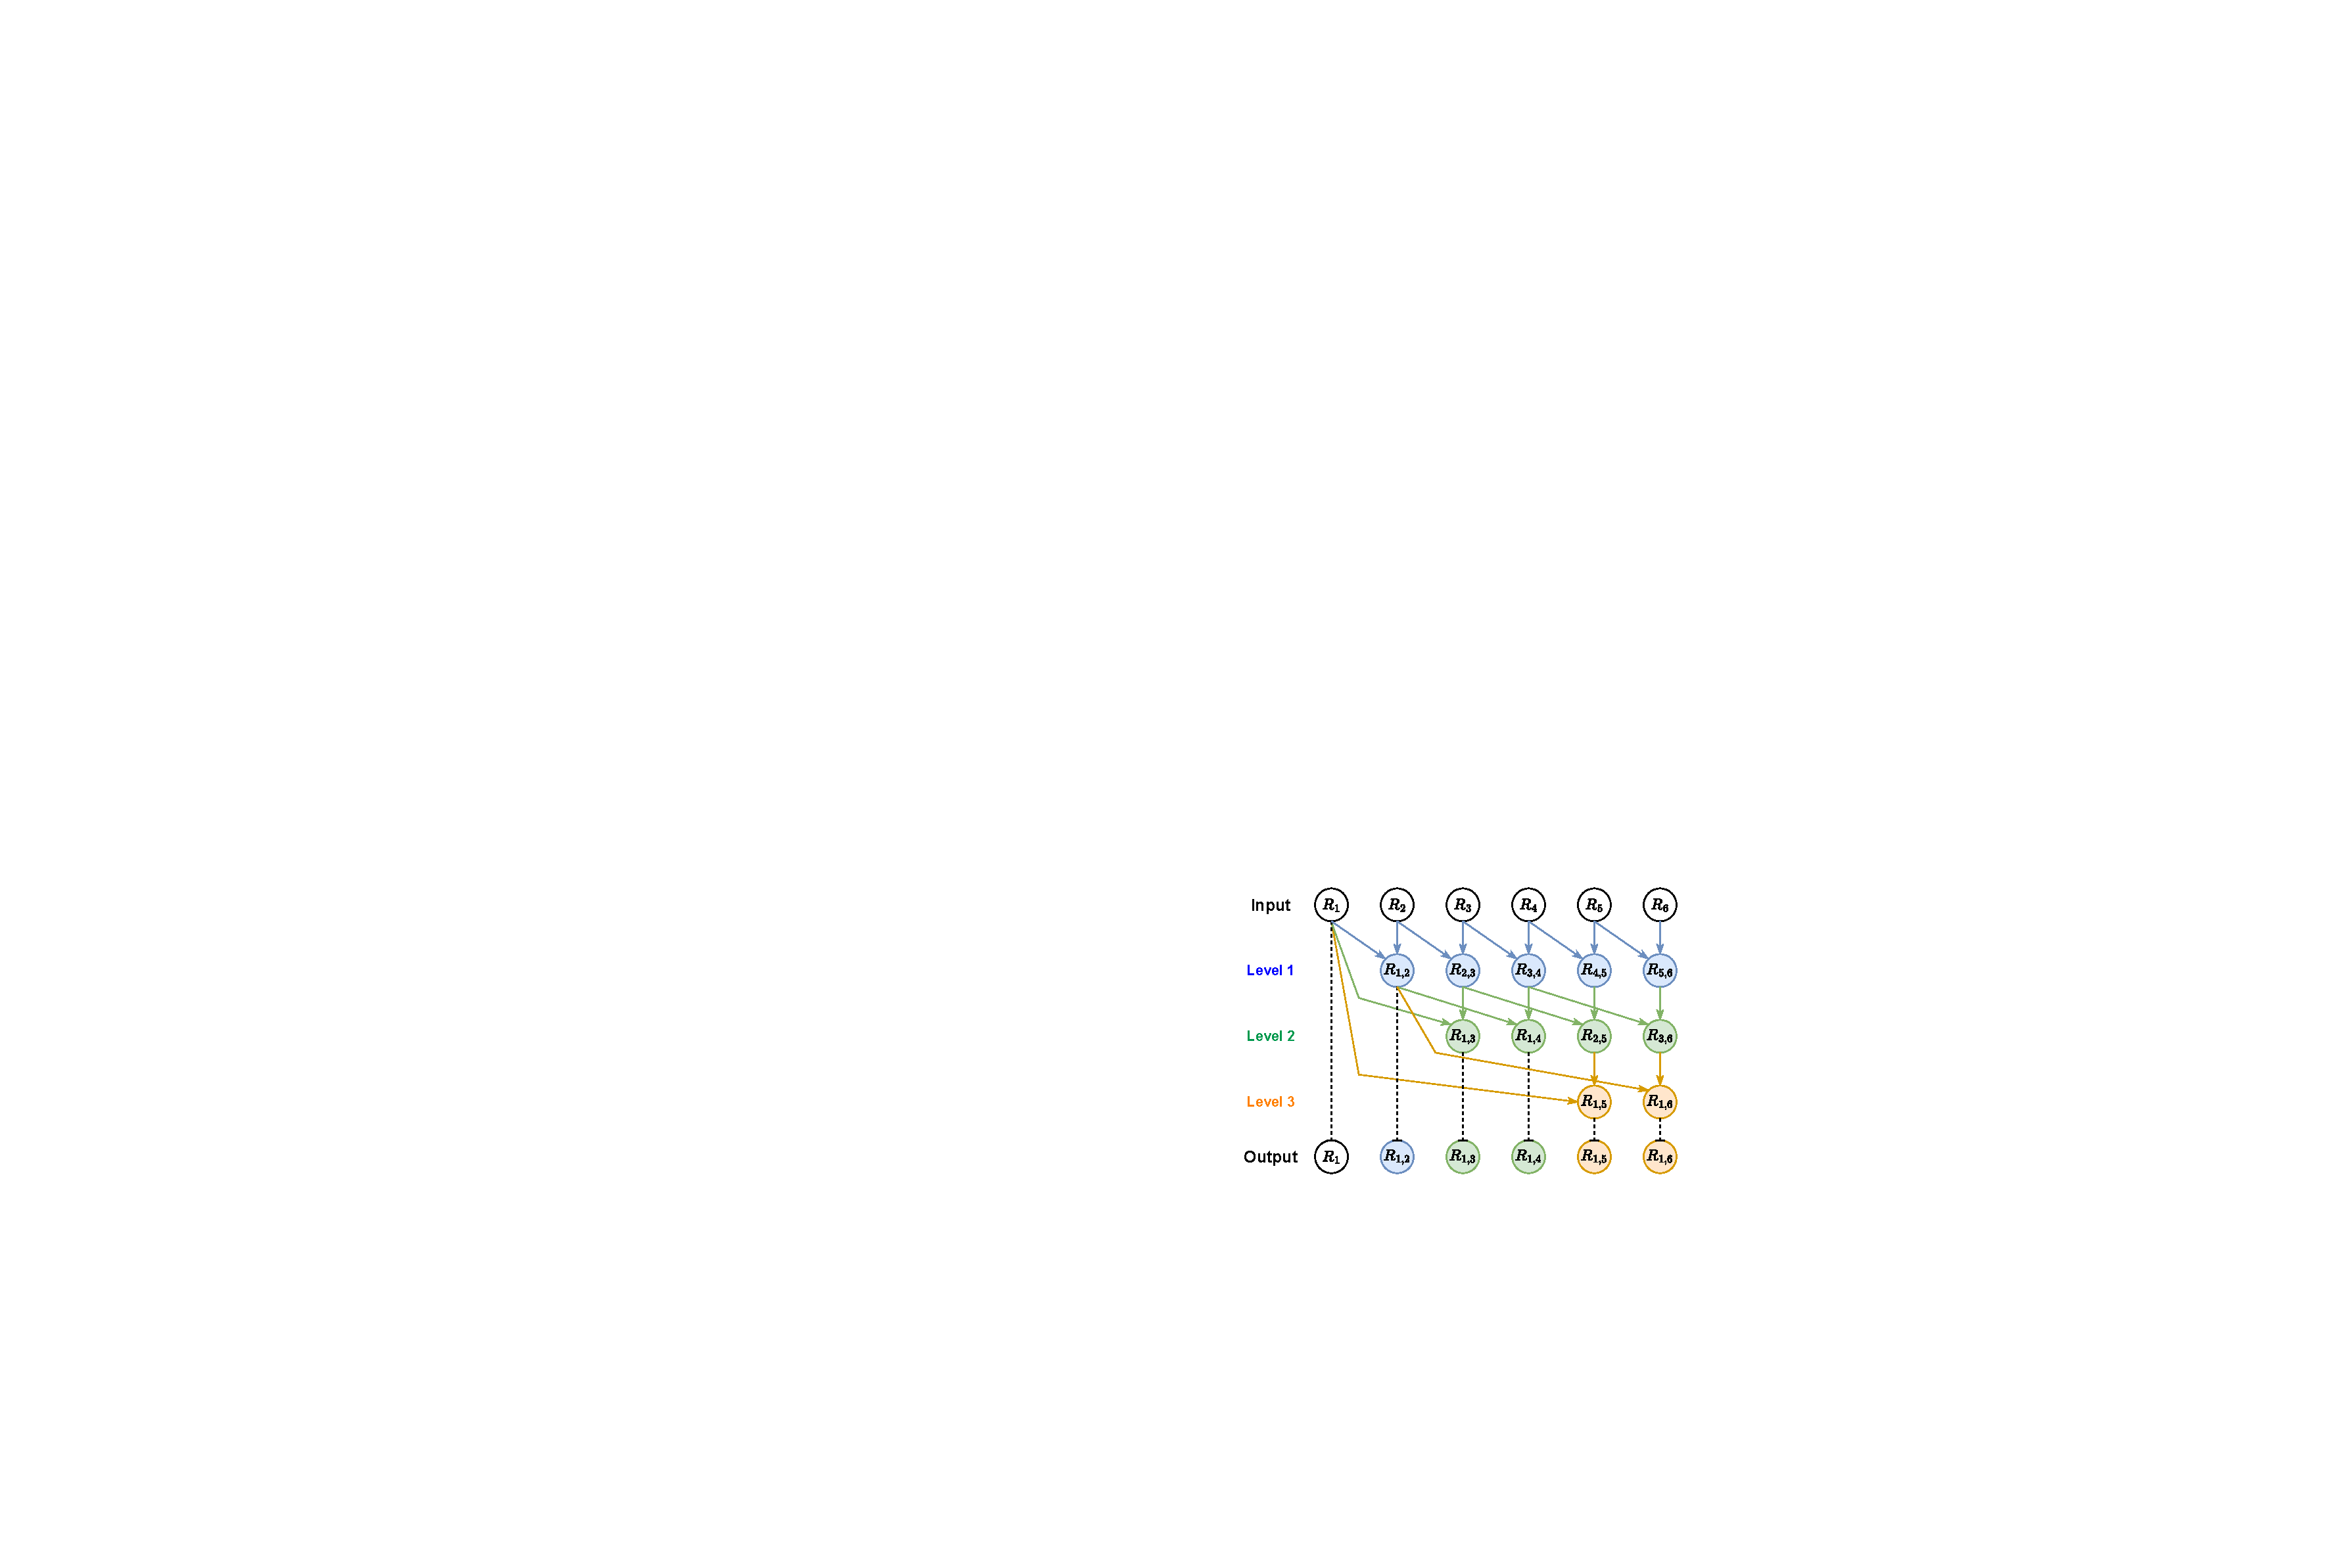
\includegraphics[width=0.95\linewidth]{tex/ch4_airimu/figs/accelerate.pdf}
    \caption{
    This graph presents the parallel scan we use to accelerate the cumulative product in our IMU integration. Given a sequence of gyroscope input from $R_1$ to $R_n$, the algorithm iterates through $\log(n)$ layers. In each layer $i$, it updates the last $N-2^i$ elements by multiplying the first $2^i$ elements. In this algorithm, each layer is a parallel batch that supports parallel computation.}
	\label{Fig:Tree}
\end{figure}

\subsection{Implementation \& Acceleration}
\label{Model: Accelerate}
In our training process, we extend the supervision period to enhance the effectiveness of the training, which is particularly crucial with high-end IMUs that only exhibit drift after long periods of integration.
While extending the training over long segments can be time-consuming, our AirIMU model addresses this challenge by fully leveraging parallel computing capabilities powered by \textit{PyTorch}.
In this section, we introduce the algorithm we designed to accelerate the cumulative product and cumulative summation to facilitate parallel computation during training.
Additionally, we reformulate the iterative covariance propagation to enable batched operation for long segments. 
These efforts not only accelerate the training process but also optimize the efficiency of real-time applications.

Specifically, the IMU preintegration and covariance propagation defined in \eqref{formula: 2.integrate} and \eqref{formula: 4.cov} relies heavily on the cumulative product of $SO3$ on manifolds and cumulative summation of the acceleration.
To accelerate the integration, we design a parallel scan algorithms as shown in \fref{Fig:Tree}, where each node represents an element in $SO3$.
In this implementation, the integration with a length of $N$ can be separated into $\log_2(N)$ iterations.
During each iteration $i$, it updates each node with the preceding node positioned $2^{i}$ place before it, which can be parallel computed.
This approach achieves $O(\log N)$ time complexity while maintaining the $O(N)$ memory usage.

Different from the segment tree strategy proposed by Brossard et al. \cite{brossard2020denoising}, which predicts only the final state $R_{1,6}$ of the gyroscope integration, our approach is designed to calculate every intermediate result throughout the integration within the same level of time.
The intermediate results significantly accelerates the calculation of the matrix of $A$, and thereby accelerates the covariance propagation.
Moreover, we not only use this approach in gyroscope integration, but also for accelerometer integration and the covariance propagation.
Overall, we integrate this algorithm into two operators: the \texttt{cumsum} for the cumulative summation and the \texttt{cumprod} for the cumulative product of the $SO3$ on manifolds.

The conventional solution outlined in \eqref{formula: 4.cov} iteratively calculates the covariance of each state.
This iterative approach, while methodically sound, requires performing covariance propagation thousands of times, even for supervising brief segments lasting a few seconds.
Such an iterative method is inefficient for training, leading to significant computational burdens. 
To address this inefficiency and fully utilize the parallel computing capabilities, we reformulate the covariance propagation for $\Sigma_{i,j}$ to two steps.

First of all, we calculate the matrix list $C^A_{i,j}$ with $\prod_{k=j}^i A_{k}$ through the \texttt{cumprod} of the matrix $A_k$,  
and the matrix list $C^B_{i,j}$ consisting the initial covariance $\Sigma_{i,i}$ and the matrix $B$.
\begin{equation}
    \begin{split}    
        C^A_{i,j} =& [\prod_{k=j}^i A_{k}, \prod_{k=j}^{i+1} A_{k},...,A_j, I_{9\times9}], \\
        C^B_{i,j} = & [\Sigma_{i,i}, B_i, ..., B_{j-1}, B_j].\\
    \end{split}
\end{equation}
Secondly, the covariance $\Sigma_{i,j+1}$ can be calculated by the product over $C^A_{i,j}$ and $C^B_{i,j}$:
\begin{equation}
    \Sigma_{i,j+1} = C^A_{i,j}  \text{diag}(C^B_{i,j})  {C^A_{i,j}}^T.
\end{equation}

With this re-implementation, we are now able to supervise the IMU integration over extended sequences. For instance, in the helicopter navigation scenario described in \sref{Exp: nearearth}, our model is trained with unusually long segments that exceed one minute in duration. This extended supervision period captures the drift inherent in the navigation-grade IMU after long-term integration, which is crucial for achieving reliable navigation in aerial environments.

\subsection{IMU-GPS PGO system}
\label{Model: System}

\begin{figure}[t]
	\centering 
    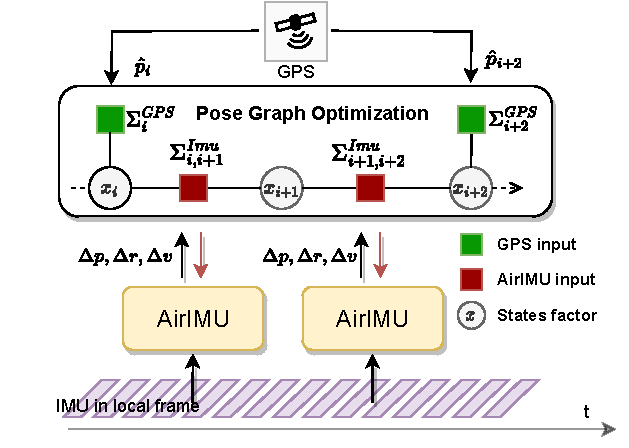
\includegraphics[width=\linewidth]{tex/ch4_airimu/figs/FigurePGO.drawio.pdf}
    \caption{Pose graph optimization of a GPS signal with IMU pre-integration. The state of the graph is defined as $x_{i}$ constrained by two different observations: IMU ($\Delta p$, $\Delta v$ and $\Delta r$) and GPS ($\hat p_i$). We back-propagate the gradient through the IMU pre-integration and covariance propagation to learn the integration and noise model.}
	\label{Fig:PGOGPS}
\end{figure}

To recover the inevitable drift from inertial odometry, auxiliary sensors like GPS are employed to fuse with the IMU measurements in the PGO.
When fusing the IMU measurements with other sensor, the covariance of the IMU integration $\Sigma_\theta(x)$, plays a critical role in the fusion.
In this section, we describe the construction of a PGO that incorporates both the AirIMU model and GPS.
We demonstrate how leveraging the learned covariance from AirIMU enhances the optimization process.
This integrated system not only compensates for the drift inherent in IMU pre-integration but also effectively utilizes the complementary sensors, resulting in more reliable and accurate navigation results.

In \fref{Fig:PGOGPS}, we show the system pipeline and the factor graph incorporating GPS signals.
The objective of the PGO is to optimize the state of the robot $x$, which is modeled as the factor in our PGO.
From the AirIMU, we take the pre-integrated increments ($\Delta p$, $\Delta v$, and $\Delta r$) as the observation.
These observations are then propagated alongside the initial state $x_i (R_i, v_i, p_i)$ to calculate the state $x_j (R_j, v_j, p_j)$, forming the basis to compute the IMU residual:

\begin{equation}
\begin{aligned}
    e^{IMU}_{ij}(\Delta v_{ij}, \Delta p_{ij}, \Delta r_{ij}) = \begin{bmatrix}
        {\Delta}R_{ij} {}^WR_i  ({}^WR_j)^{-1} \\
       {}^Wv_i + {}^WR_i * {\Delta}v_{ij}  - {}^Wv_j\\
         {}^Wp_i + {}^WR_i * {\Delta}p_{ij}  - {}^Wp_j
    \end{bmatrix}.\\
\end{aligned}
\end{equation}

To calculate the corresponding covariance matrix $\Sigma^{IMU}_{ij}$ of the IMU integration. 
We leverage the predicted uncertainty from the network $[\eta^{acc}_k, \eta^{gyro}_k] = \Sigma_\theta(w, a)$ and employ it in \eqref{formula: 4.cov} to propagate the covariance matrix $\Sigma^{IMU}_{ij}$.
Since the initial state $x_i$ is updated after each optimization, we also update the corresponding covariance $\Sigma_{i,i}$ of the $i^{th}$ state during the optimization.
This ensures the covariance of the state is bounded, giving the other sensors' measurements and advancing the reliability.

We define the GPS signal as $\hat p_i \in R^3$ to constrain the state of position ${}^Wp_i$, where the residual of GPS measurements are:
\begin{equation}
e^{GPS}_i( {}^W \hat p_i) = {}^W \hat p_i -  {}^Wp_i 
\end{equation}
where the measurement of the GPS is $\hat {}^Wp_i$ with a corresponding covariance matrix defined as a diagonal matrix $\Sigma^{GPS}_i$.
The optimization with both the $e^{GPS}_i(\hat p_i)$ and $e^{IMU}_{ij}(\Delta v_{ij}, \Delta p_{ij}, \Delta r_{ij})$ can be formulated as:
\begin{equation}
X^* = \argmin_{X}\left\{ \sum_{k\in G} \|e^{GPS}_k\|^2_{\Sigma^{GPS}_k} +  \sum_{l \in L} \| e^{IMU}_l \|^2_{\Sigma^{IMU}_l} \right\}
\end{equation}
where $G$ and $L$ is the set of GPS and IMU observations and the $X$ is the factor. We can solve this optimization by Levenberg-Marquardt algorithms.

\section{Experiments}

\begin{table}[!t]
    \caption{Dataset summary showing the comprehensive evaluation across different IMU grades and platforms}
    \centering
    \resizebox{\linewidth}{!}{
    \begin{tabular}{l|llll}
        \toprule
        \textbf{Datasets} & \textbf{Duration} & \textbf{IMU} & \textbf{Modality}\\
        \midrule
        EuRoC \cite{burri2016euroc}   & 22m29s & ADIS16448 & Drone \\ 
        TUM-VI \cite{schubert2018tum}  & 13m31s  & BMI160 & Handheld\\
        SubtMRS \cite{zhao2023subt} & 2h52m  & Epson M-G365 & Ground robot\\
        KITTI \cite{KITTIDataset}  & 43m44s  & OXTS RT 3000 & Vehicle \\
        ALTO \cite{hemann2016long} & 2h12m  & NG LCI-1 & Helicopter\\
        \bottomrule
        \end{tabular}
        \label{datasets}
    }
\end{table}

As shown in \fref{Fig:Devices}, we comprehensively evaluate our method across a full spectrum of IMUs, from low-cost automotive-grade to high-end navigation-grade IMUs, each featured on different platforms and modalities. 
The price and gyro in-run bias stability are plotted, revealing a clear correlation between cost and performance stability.
At the high end of the spectrum, we have the \texttt{NG LITEF LCI-1} in the ALTO dataset \cite{cisneros2022alto} with a cost exceeding \$50,000, showcasing exceptional bias stability in helicopters.
The tactical-grade IMUs, like the \texttt{OXTS RT3003} in the KITTI dataset \cite{KITTIDataset} and the \texttt{Epson M-G365} in the Subt-MRS \cite{zhao2023subt}, are priced at approximately \$25,000 and \$1,400, deployed on UGVs and vehicles respectively.
On the low-cost end, we feature the industrial-grade IMU \texttt{BMI 160} on drones at around \$500 and the automotive-grade IMU \texttt{ADIS 16448} at \$3 used in handheld platforms, demonstrating the feasibility of using low-cost IMUs for certain applications.
These datasets evaluate the adaptability of our model not only across multiple grades of IMUs but also across various platforms and modalities.

In our experiments, we demonstrate the dual purposes of the AirIMU: state estimation and uncertainty estimation.

\textbf{State Estimation:}
We demonstrate the AirIMU model's superior performance in IMU integration, outperforming both learning-based IMU de-noising algorithms and traditional IMU calibration algorithms.
Notably, the AirIMU model achieves a tenfold increase in accuracy compared to learning-based inertial odometry methods in short-term integration.
We also demonstrate the potential of the AirIMU model in GPS-denied helicopter navigation using high-end IMUs. 
This assessment spans a cruising distance over 262 \si{\km}, providing a realistic and challenging environment for evaluating our method.

\textbf{Learned Uncertainty:}
We assess our model with a particular emphasis on the potency of the learned uncertainty.
An ablation study focused on a GPS-PGO experiment reveals an average improvement of 31.6\% in utilizing the learned uncertainty.
Furthermore, we conduct an ablation study to highlight the benefits of jointly training the uncertainty module with the IMU noise correction.
This dual training approach significantly improves the network's ability to extract features from IMUs, resulting in a performance enhancement of 17.8\% compared to models solely trained on noise correction.

\subsection{Evaluation Metrics}

We define the following metrics to evaluate the performance of our model over assigned time intervals:

\textbf{Rotational Root Mean Squared Error} (R-RMSE, \si{\radian}),
\begin{equation}
     \text{R-RMSE} = \sqrt{\frac{1}{N} \sum^N_{i=1}\left\| \log\left(\hat{R}_{i,i+\Delta t}^T R_{i,i+\Delta t}\right)\right\|^2_2},
\end{equation}
calculates the RMSE of the rotations over the assigned time intervals on the manifold space.

\textbf{Positional Root Mean Squared Error} (P-RMSE, \si{\meter})
\begin{equation}
    \text{P-RMSE} =\sqrt{ \frac{1}{N}\sum^N_{i=1}\left\| p_{i+\Delta t} - p_{i} - R_{i}\hat{R}_{i}^T \left(\hat{p}_{i+\Delta t} - \hat{p_{i}}\right)\right\|^2_2},
\end{equation}
calculates the RMSE of the relative displacements over the assigned time intervals.

\begin{figure}[!t]
	\centering
    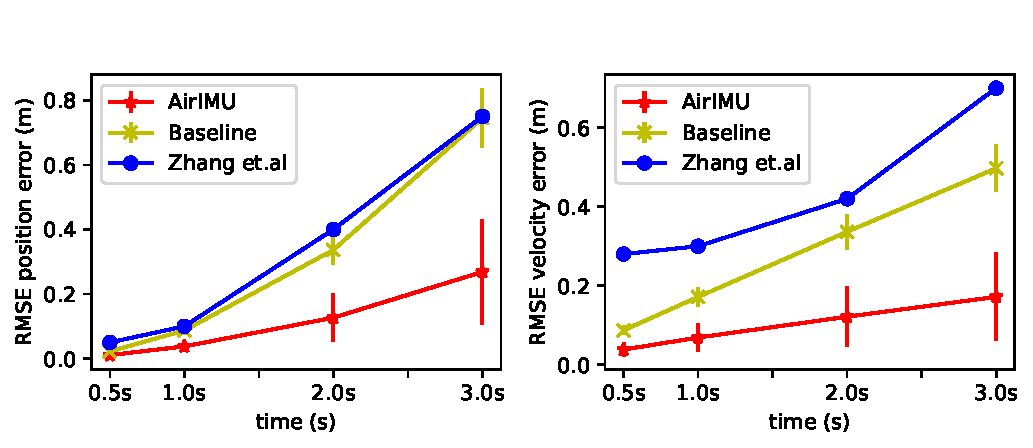
\includegraphics[width=\linewidth]{tex/ch4_airimu/figs/FigIntegrate.pdf}
    \caption{Integration results comparison showing AirIMU performance across different integration periods and datasets. AirIMU consistently outperforms baseline methods across various IMU grades and integration durations.}
	\label{Fig:Integration}
\end{figure}

\begin{figure}[!t]
	\centering
    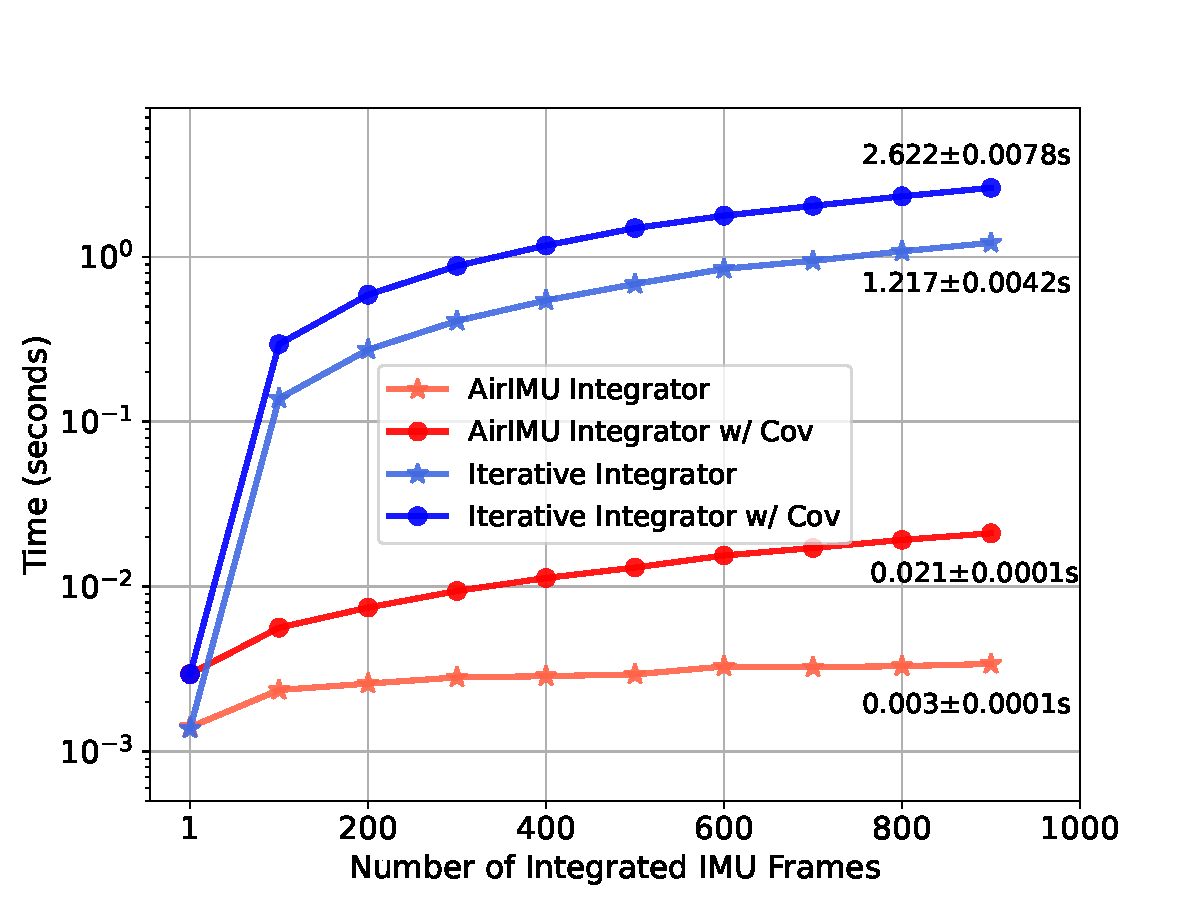
\includegraphics[width=\linewidth]{tex/ch4_airimu/figs/TimeAnalysis.pdf}
    \caption{Time analysis of the AirIMU integrator compared to iterative methods. We integrate IMU input with different lengths (from 1 frame to 1000 frames) and display the time consumption on a log scale. The AirIMU integrator demonstrates a hundredfold improvement in efficiency.}
	\label{Fig:TimeAnalysis}
\end{figure}

\subsection{IMU Integration Performance}

\fref{Fig:Integration} shows comprehensive integration results across all evaluated datasets. AirIMU consistently outperforms traditional calibration methods and learning-based approaches across different IMU grades and integration periods. The method shows particular strength in:

\begin{itemize}
\item \textbf{Cross-IMU Adaptability}: Superior performance across automotive-grade to navigation-grade IMUs
\item \textbf{Long-term Integration}: Reduced drift accumulation over extended periods
\item \textbf{Real-world Robustness}: Effective handling of environmental disturbances and non-deterministic errors
\end{itemize}

\subsection{Computational Efficiency}

\fref{Fig:TimeAnalysis} demonstrates the computational advantages of our parallel implementation. The differentiable integrator with parallel scan algorithms achieves:

\begin{itemize}
\item \textbf{100x speedup} compared to iterative covariance propagation methods
\item \textbf{O(log N) complexity} for cumulative operations through tree-structured algorithms
\item \textbf{Batched processing} enabling efficient training on long sequences
\end{itemize}

\subsection{GPS-IMU Pose Graph Optimization}

\begin{figure}[!t]
	\centering
    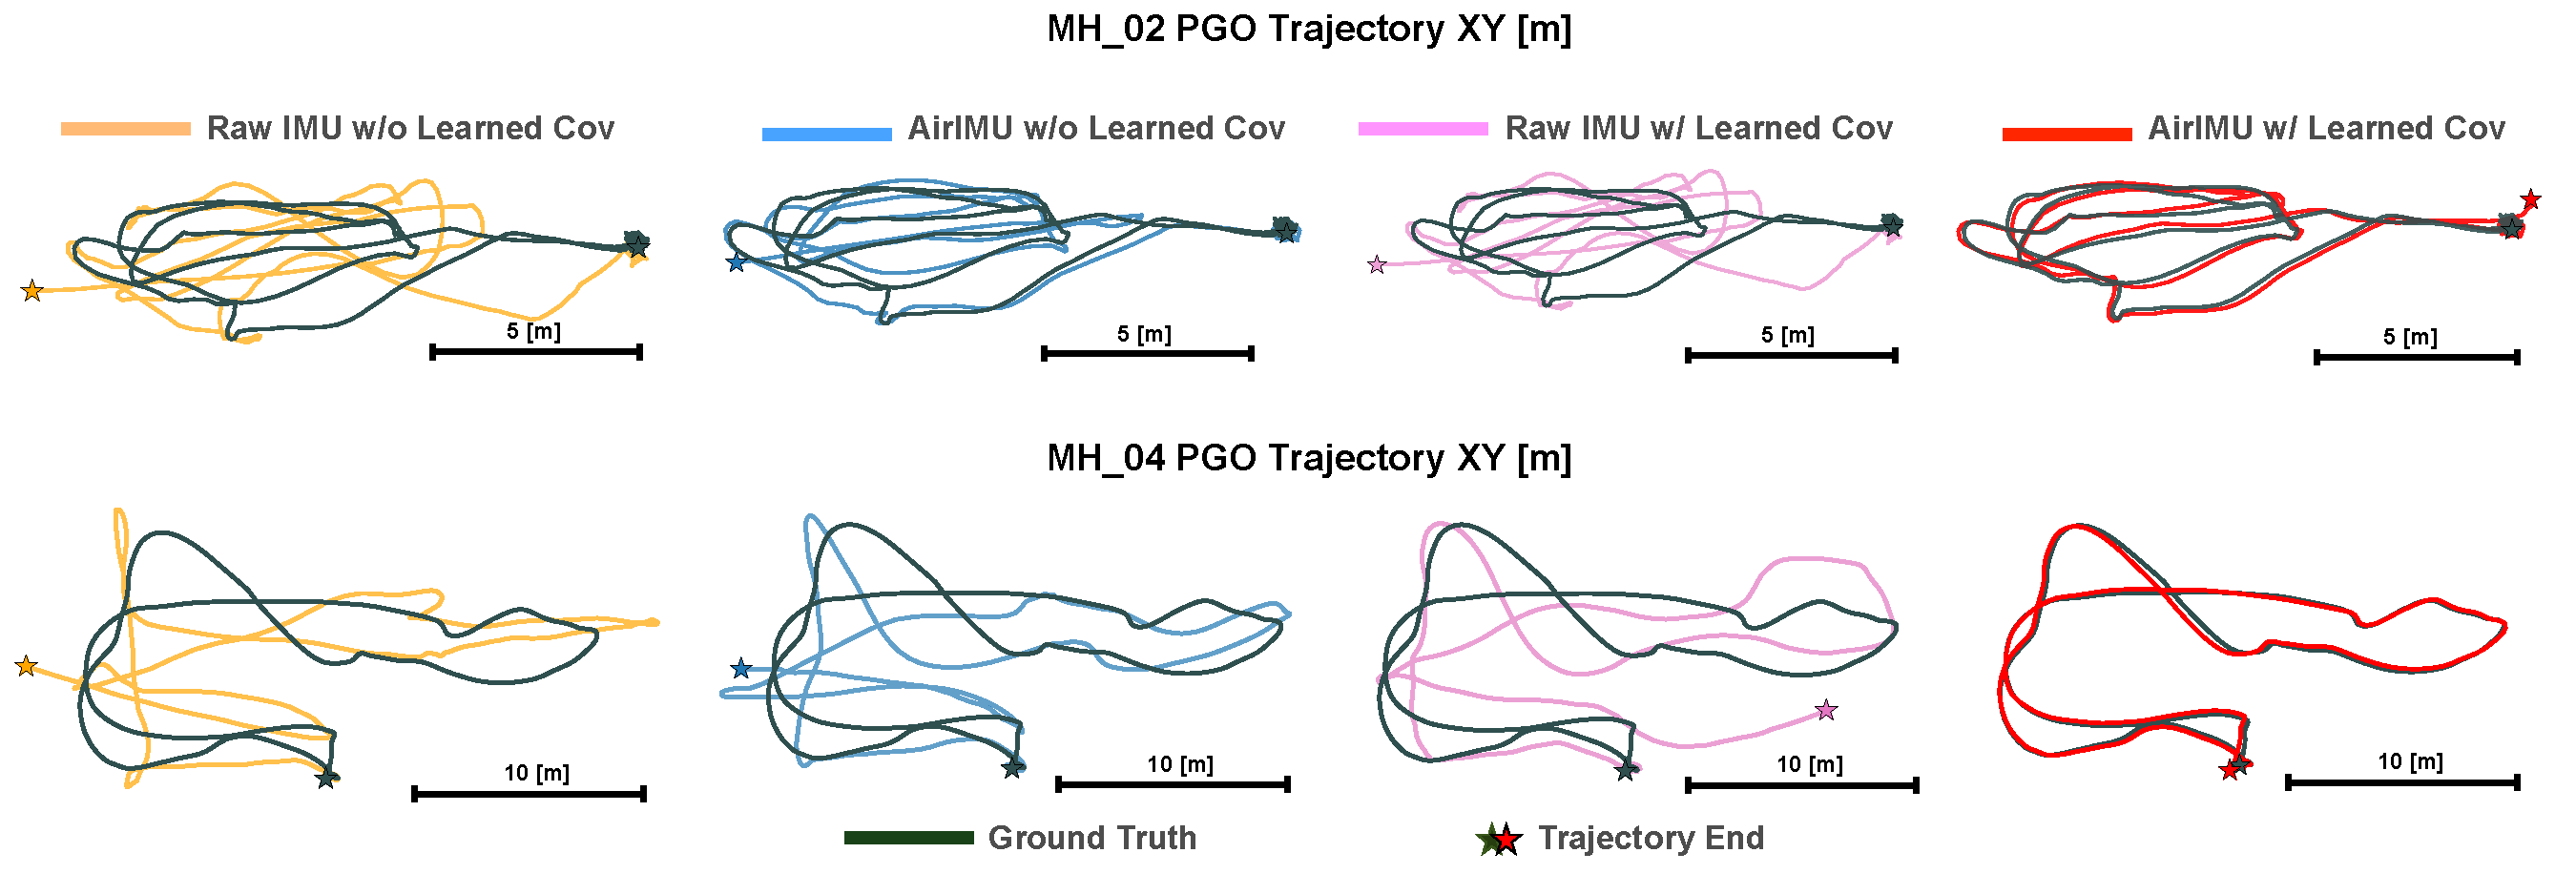
\includegraphics[width=\linewidth]{tex/ch4_airimu/figs/PGO_Visualize.pdf}
    \caption{PGO results visualization showing the effectiveness of learned uncertainty in GPS-IMU fusion. The learned covariance from AirIMU enables more accurate and robust optimization compared to fixed uncertainty models.}
	\label{Fig:PGOResults}
\end{figure}

The integration with GPS through pose graph optimization (\fref{Fig:PGOResults}) validates the effectiveness of learned uncertainty models. Key results include:

\begin{itemize}
\item \textbf{31.6\% improvement} in GPS-IMU fusion accuracy using learned covariance
\item \textbf{Adaptive uncertainty}: Dynamic adjustment to sensor conditions and environmental factors
\item \textbf{Robust optimization}: Better convergence and stability in challenging scenarios
\end{itemize}

\subsection{Large-Scale Navigation Evaluation}
\label{Exp: nearearth}

\begin{figure}[!t]
	\centering
    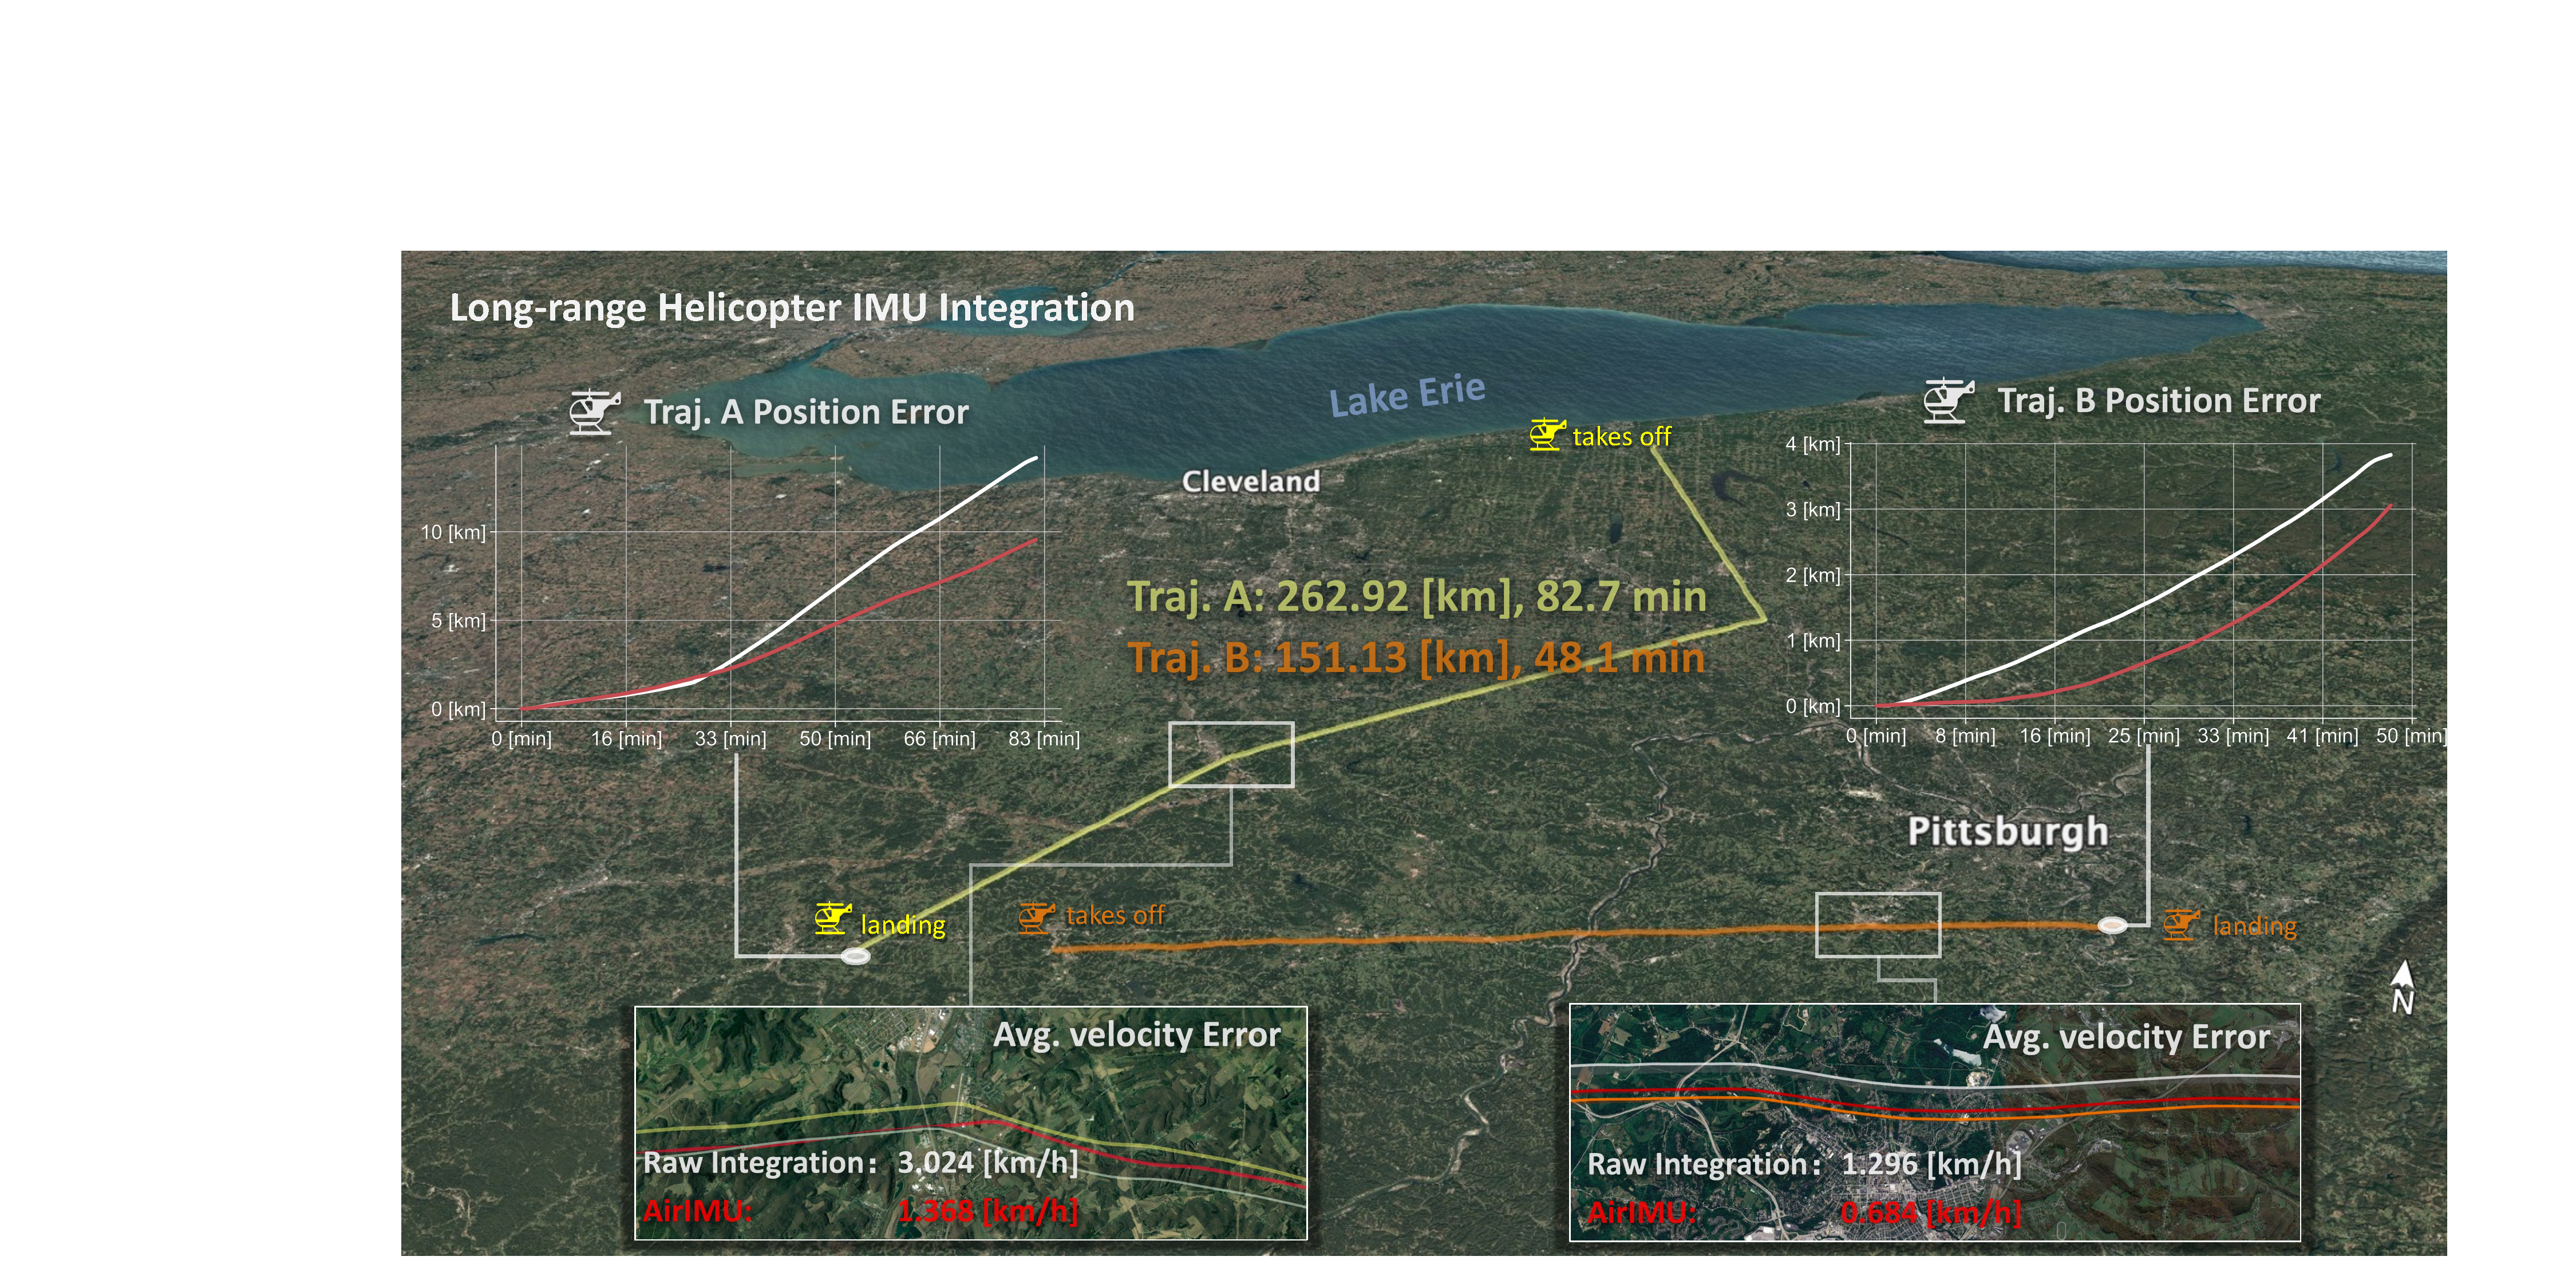
\includegraphics[width=\linewidth]{tex/ch4_airimu/figs/Fig_nearearth3.pdf}
    \caption{Near-earth helicopter navigation trajectory visualization over 262 km using navigation-grade IMUs. AirIMU enables precise long-term navigation in GPS-denied environments.}
	\label{Fig:NearEarth}
\end{figure}

The helicopter navigation evaluation (\fref{Fig:NearEarth}) on the ALTO dataset demonstrates AirIMU's capability for large-scale, long-duration navigation:

\begin{itemize}
\item \textbf{262 km trajectory}: Extended navigation without GPS dependency
\item \textbf{Navigation-grade IMU}: Effective utilization of high-end sensor capabilities
\item \textbf{Real-world conditions}: Robust performance under aerial navigation challenges
\end{itemize}

\section{Limitation and Discussion}

We propose a hybrid method that can adapt to a full spectrum of IMUs. However, we've observed that the AirIMU model trained on a single IMU does not readily generalize to a different IMU with different specifications and operating frequencies.
For instance, a model trained for the tactical-grade IMU \texttt{Epson G365}, used in the SubT-MRS dataset, does not apply to the automotive-grade IMU \texttt{ADIS16448} in the TUMVI dataset due to their different physical design.
Our current model is specialized, focusing on a single IMU's unique noise profile and uncertainty characteristics rather than attempting to create a one-size-fits-all model.
If we need to deploy the AirIMU model to a new type of IMU, fine-tuning with new IMU data is necessary.

In the future, we may explore the potential for generalizing through different sensors within the same models or types of IMUs.
For example, whether the sensor model trained on one \texttt{Epson G365} can be adapted to other \texttt{Epson G365} IMUs, potentially a more versatile application to scale up in manufacturing the same types of IMU.

\section{Conclusion}

We propose AirIMU, a hybrid IO system with a differentiable integrator and covariance propagator. 
To demonstrate the efficacy of the learned covariance model, we conduct an ablation study on a GPS PGO experiment, revealing that the learned covariance decreased the loss of PGO by 31\%. 
We evaluate our model in all spectrums of IMUs' grades, spanning the entry-level IMUs (Automotive Grade) to the high-end IMUs (Navigation Grade). 
Our experiments demonstrate that the AirIMU model achieves outstanding performance across the board. The evaluation also includes IMUs operating in a wide range of environments and featuring multiple agent modalities. 
We find that AirIMU not only excels at regular indoor environments but also performs well with a ground vehicle dataset over 2 \si{km} and a large-scale helicopter dataset over 414 \si{km}.
Additionally, we open-source the differentiable IMU integrator and the covariance propagation, which is implemented in the \textit{PyPose} framework.
Given these advancements, we are optimistic that the proposed method can provide a strong foundation for further research in inertial navigation systems and multi-sensor fusion.